%!TEX root=../main.tex
\section{Performance Evaluation}
\label{sec:eval}

In this section, we present the end-to-end evaluation (\S\ref{ssec:e2e-performance}) and the analysis of three design principles (\S\ref{subsec:eval-disaggregated}–\ref{subsec:eval-reward-worker}). 

\begin{figure*}[tb]
    \centering
    \begin{subfigure}[b]{0.466\linewidth}
        \centering
        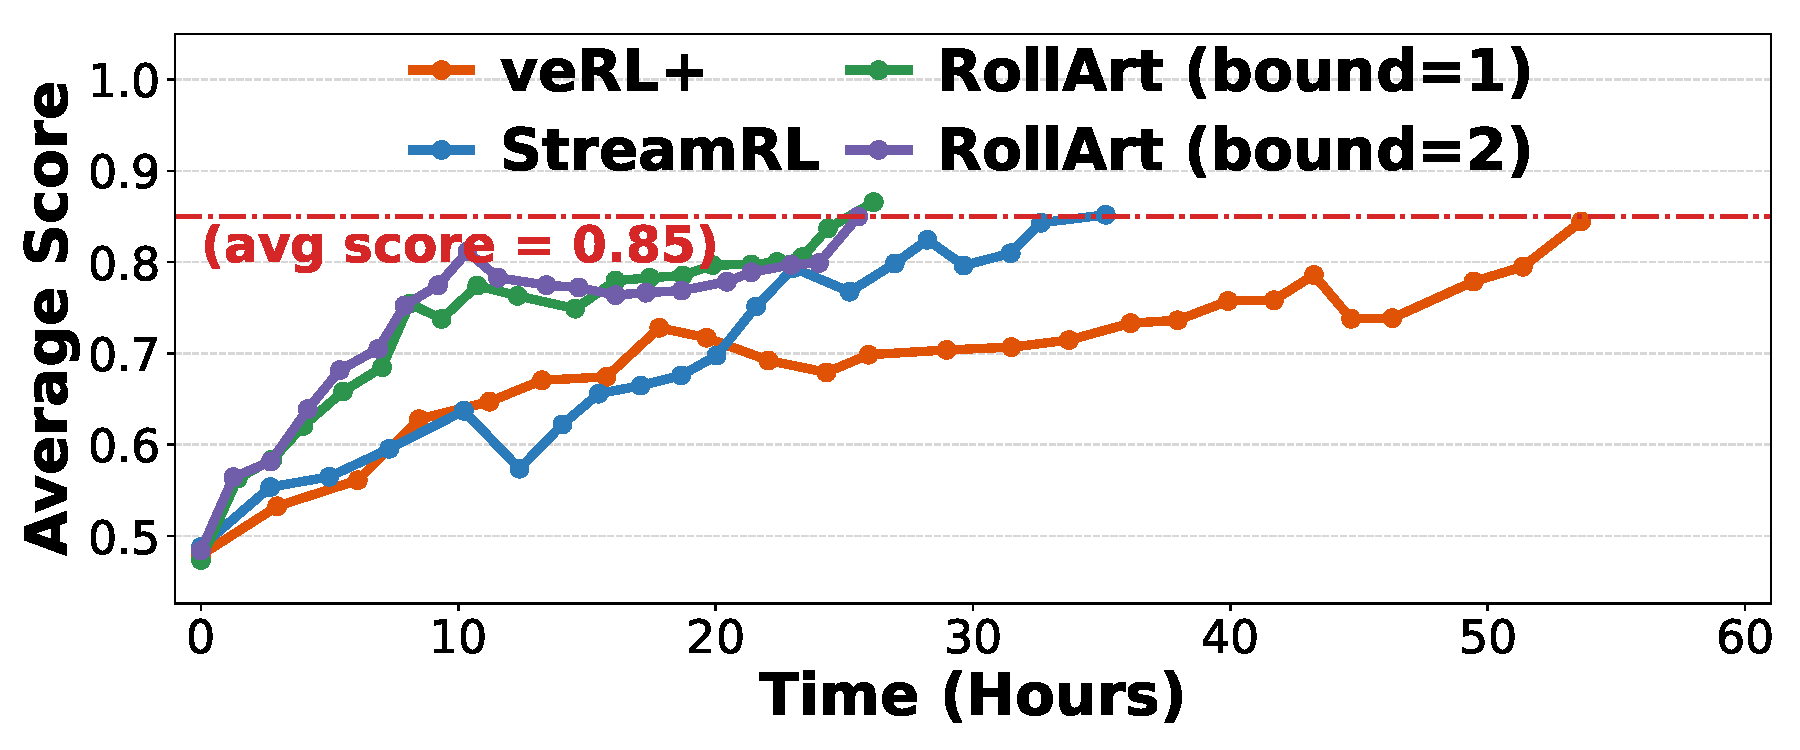
\includegraphics[width=\linewidth]{figs/e2e/score_comparison.pdf}
        \caption{Time-to-score.}
        \label{fig:e2e-acc}
    \end{subfigure}
    \begin{subfigure}[b]{0.31\linewidth}
        \centering
        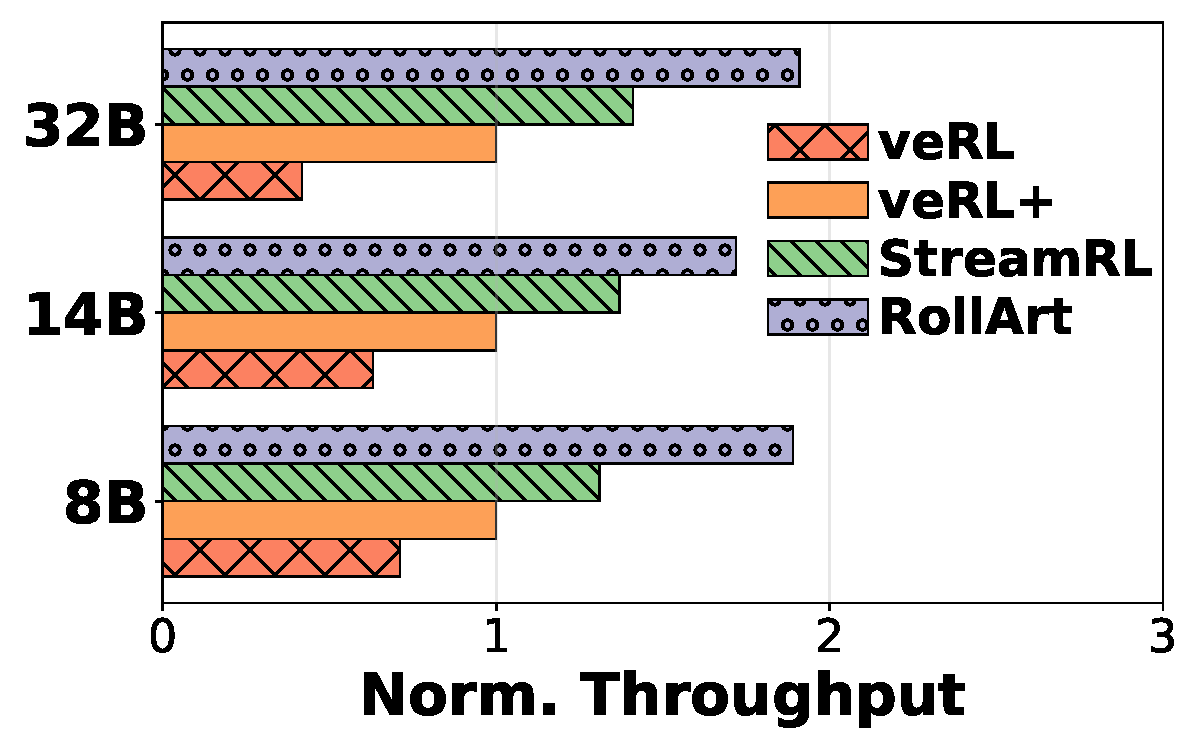
\includegraphics[width=\linewidth]{figs/e2e/modelsize_thr_horizontal.pdf}
        \caption{Throughput Efficiency.}
        \label{fig:e2e-thr}
    \end{subfigure}
    \begin{subfigure}[b]{0.214\linewidth}
        \centering
        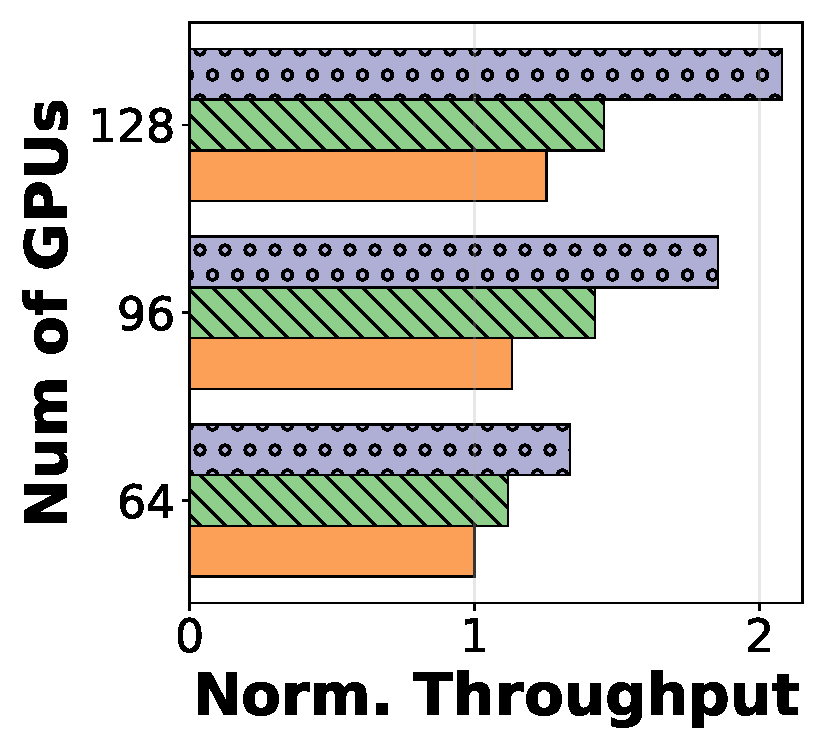
\includegraphics[width=\linewidth]{figs/e2e/modelsize_scaling_horizontal.pdf}
        \caption{Resource Scaling.}
        \label{fig:e2e-thr-scaling}
    \end{subfigure}


    \caption{
        Comparison of (a) end-to-end time-to-score on Qwen3-32B;
        (b) normalized throughput across LLMs for different approaches; and (c) normalized throughput of Qwen3-14B across different numbers of H800 GPUs.
    }
    \label{fig:e2e-combined}
    \vspace{-10pt}
\end{figure*}


\subsection{Evaluation Setup}

\noindent\textbf{Models and Tasks.} 
We train Qwen3~\cite{yang2025qwen3technicalreport} LLM family (8B–32B) on a diverse mixture of agentic tasks (\autoref{tab:env-taxomy}). All models are configured with a maximum context length of 32K tokens. Due to the difficulty of the \texttt{SWE-bench} agentic task, we train it only on Qwen3-32B. we employ a 7B reward LLM to validate the reasoning process of mathematical task. 


\noindent\textbf{Training Configurations.} We use the GRPO algorithm~\cite{he2025deepmath} with a training batch size of 512, a group size of 8, and a uniform sampling ratio across all tasks. For asynchronous training, we allocate 32 H800 GPUs to the training stage and use the remaining H20 and H800 GPUs for rollouts. During rollout, the tensor-parallelism degrees for Qwen3-8B/14B/32B are set to 1, 2, and 4, respectively, and we tune the training parallelism to maximize throughput. We run rollouts on vLLM 0.8.4 and training on Megatron v0.12.2, with prefix caching and CUDA graphs enabled during rollout.


\noindent\textbf{Weight Update Engine.} We use NCCL~\cite{nccl} v2.26.5 to perform intra-cluster weight update and Mooncake v0.3.7~\cite{qin2024mooncake} storage server for cross-cluster communication. 

\noindent\textbf{Hardwares.} \SystemName{} is deployed on an H800 cluster with 96 GPUs and an H20 cluster with 32 GPUs. Within each cluster, GPU nodes are connected via 400 Gbps InfiniBand, while cross-cluster communication uses a 200 Gbps Ethernet network. We use a dedicated CPU cluster for \texttt{SWE-bench} and another for the remaining environments. The reward workers run on our internal serverless platform. Without clarification, all experiments are performed with 128 GPUs. 

\noindent\textbf{Baselines.} Since no existing open-source system supports our full spectrum of agentic tasks, we follow the synchronous RL implementation of veRL (\textbf{veRL}). To strengthen this baseline, we additionally enable asynchronous reward computation, asynchronous environment interaction, and \textit{Reward-as-a-Service}, and denote this as \textbf{veRL+}. We also compare against StreamRL~\cite{StreamRL} and enable the one-off training paradigm~\cite{deepscaler2025} (see \autoref{fig:paradigm-all-in-one}-Left), which parallelizes rollout and training by consuming trajectories generated in the previous step. The optimizations used in veRL+ are also applied to StreamRL. We use Megatron~\cite{shoeybi2019megatron} for the training stage, which does not support heterogeneous GPU configurations. StreamRL likewise does not support heterogeneous GPUs during rollout. For simplicity, we run both baselines on 128 H800 GPUs; consequently, \SystemName{} incurs roughly 83\% of the baselines’ per-GPU-hour cost.

\noindent\textbf{Metrics.} We measure end-to-end latency as the average step time over five iterations. The throughput is the total number of prompt and response tokens in a global batch by the step time~\cite{sheng2025hybridflow}. We report average validation score across all tasks.



\subsection{End-to-End Evaluation}
\label{ssec:e2e-performance}


\noindent\textbf{Model Convergence.} We measure the score per ten iterations and report time-to-score with a target score of 0.85 in \autoref{fig:e2e-acc}. StreamRL achieves a 1.52\(\times\) end-to-end latency speedup over the veRL+ baseline by overlapping training and rollout. \SystemName{} keeps the rollout GPUs saturated by launching more rollouts and reusing partially generated trajectories across iterations. Consequently, with a bound of 1, the asynchronous approach delivers a 2.05\(\times\) and 1.35 \(\times\) step time reduction over the veRL+ and StreamRL. Although the asynchronous configuration with a bound of 2 exhibits a faster initial convergence rate, it results in a slightly worse time-to-score than the bound of one at later stages. Overall, different bounds still provide satisfactory convergence performance.

\noindent\textbf{Throughput Efficiency.} We present the throughput efficiency of different approaches in \autoref{fig:e2e-thr}. We normalize the throughput results to veRL+ baseline. We set the bound to 1 for \SystemName{}. The optimization techniques including asynchronous reward and envinvornment interaction as well as serverless reward worker can improve 1.40-2.40\(\times\) throughput. By overlapping rollout and training stage, we can see StreamRL achieves 1.31-1.47\(\times\) throughput increase. By fine-grained ascynrhony, \SystemName{} can provide 2.65-4.58\(\times\) throughput over the Sync baseline. Overall, \SystemName{} achieves substantial advantages in throughput efficiency.



\noindent\textbf{Resource Scaling.} We further evaluate the resource scaling performance of \SystemName{}. Specifically, we conduct experiments on 128 H800 GPUs and vary the number of GPUs allocated to rollout from 64 to 128 for different approaches. \autoref{fig:e2e-thr-scaling} reports the normalized throughput to veRL+ baseline running on 64 H800 GPUs. As the number of allocated GPUs increases, the marginal throughput gains diminish for veRL+ and StreamRL. However, the asynchronous RL training in \SystemName{} continues to yield 1.33-2.08\(\times\) throughput improvements, demonstrating superior resource scaling efficiency. 



\subsection{Analysis of Hardware Affinity}
\label{subsec:eval-disaggregated}

\begin{figure}[tb]
    \centering
    \begin{subfigure}{0.47\linewidth}
        \centering
        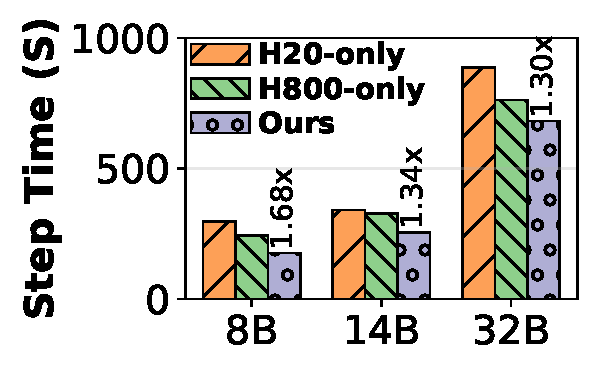
\includegraphics[width=\linewidth]{figs/col_dis/hw_affinity_3bars_small.pdf}
        \caption{Rollout Efficiency.}
        \label{fig:compute-efficiency}
    \end{subfigure}
    \begin{subfigure}{0.47\linewidth}
        \centering
        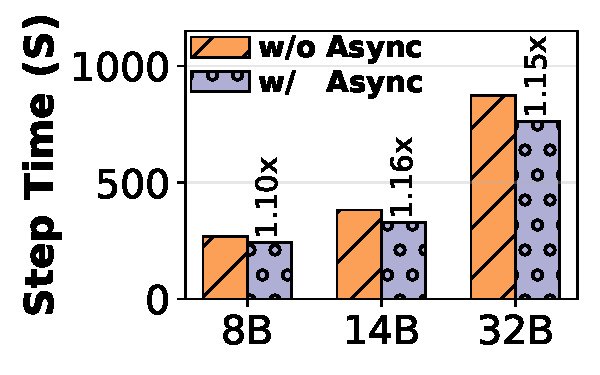
\includegraphics[width=\linewidth]{figs/col_dis/synctime.pdf}
        \caption{Cross-Cluster Comm.}
        \label{fig:comm-efficiency}
    \end{subfigure}
    % \vspace{-10pt}
    \caption{ \textbf{[Principle 1]}: (a) The efficiency of hardware affinity; (b) The benefit of async cross-cluster communication.}
    \label{fig:rollout_col_disagg}
    % \vspace{-10pt}
\end{figure}

% Rollout time for running different LLMs on a homogeneous H20 cluster, a homogeneous H800 cluster, and a heterogeneous cluster.

\noindent\textbf{Training Efficiency.} We evaluate the training efficiency on compute-optimized and bandwidth-optimized hardware across LLMs. To isolate the impact of hardware affinity, we fix the training allocation to 32 H800 GPUs and use three resource configurations for rollout: 72 H800 GPUs as the H800-only baseline, 208 H20 GPUs as the H20-only baseline, and an affinity-aware setting with 64 H800 GPUs plus 24 H20 GPUs. In the affinity-aware setup, mathematical and game-oriented agentic tasks are prioritized routed to H20 GPUs. As shown in \autoref{fig:compute-efficiency}, \SystemName{} achieves a 1.30–1.68\(\times\) step time speedup across LLM sizes compared to H20-only configuration and 1.12-1.37 speedup compared to H800-only configuration due to more H20 GPU scan reduce resource contention and benefit to decoding heavy tasks. The H20-only configuration performs worst, suggesting that many agentic tasks benefit more from compute-optimized GPUs due to frequent prefill operations. Overall, exploiting the complementary strengths of heterogeneous hardware for rollout is crucial for improving training efficiency.


\noindent\textbf{Async Cross-cluster Communication.} Hardware affinity introduces cross-cluster weight update, where Ethernet-connected clusters incur high communication overhead. In contrast to veRL’s NCCL-based communication, which assumes that all GPU servers are connected with uniformly high-bandwidth links, our setting must explicitly handle heterogeneous interconnects. \autoref{fig:comm-efficiency} compares the end-to-end step time of our asynchronous cross-cluster communication with veRL’s approach. The asynchronous communication technique achieves a 1.10-1.16\(\times\) reduction in end-to-end step time across LLMs, indicating that cross-cluster communication overhead deserves dedicated optimization.


% Here, we evaluate how asynchronous cross-cluster communication can hide the heavy cross-clsuter weight transfer. To emphasize the gains of this technique, we 

% ethernet

% \SystemName{} introduce asynchronous cross-cluster communication to prevent the low-bandwidht links a

% We evaluate our cross-cluster communication optimizations against veRL’s NCCL-based cross-cluster communication as the baseline. Specifically, we train Qwen3-8B on a rollout cluster with 8 H800 and H20 GPUs connected via 200 Gbps TCP, using a batch size of 32. \autoref{fig:comm-efficiency} reports the end-to-end step time. We observe that the optimized cross-cluster communication achieves a 1.10–1.16\(\times\) reduction in end-to-end latency across different LLMs, confirming its effectiveness.



\begin{figure}[tb]
    \centering
    \begin{subfigure}{0.23\textwidth}
        \centering
        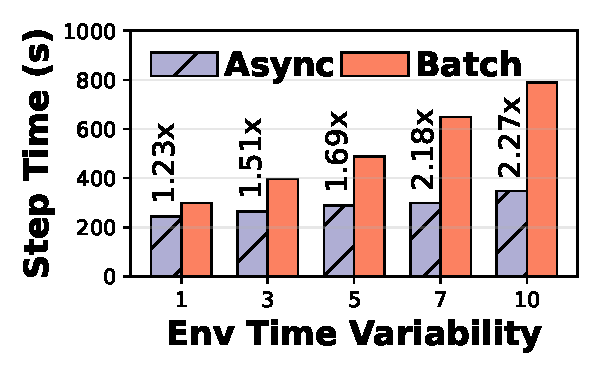
\includegraphics[width=\linewidth]{figs/async_env/async_env_time_var_bar.pdf}
        \caption{Env Time Variability.}
        \label{subfig:async_env_batch}
    \end{subfigure}
    \begin{subfigure}{0.23\textwidth}
        \centering
        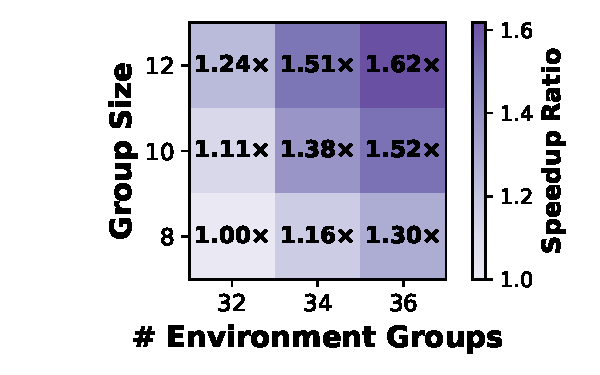
\includegraphics[width=\linewidth]{figs/async_env/async_env_redunant.pdf}
        \caption{Redundant Env Rollout.}
        \label{subfig:env-red-rollout}
    \end{subfigure}
    \vspace{-5pt}
    \caption{\textbf{[Principle 2]}: Benefits of trajectory-level Env.}
    \label{fig:rollout_env_async}
    % \vspace{-10pt}
\end{figure}




\begin{figure}[tb]
    \centering
    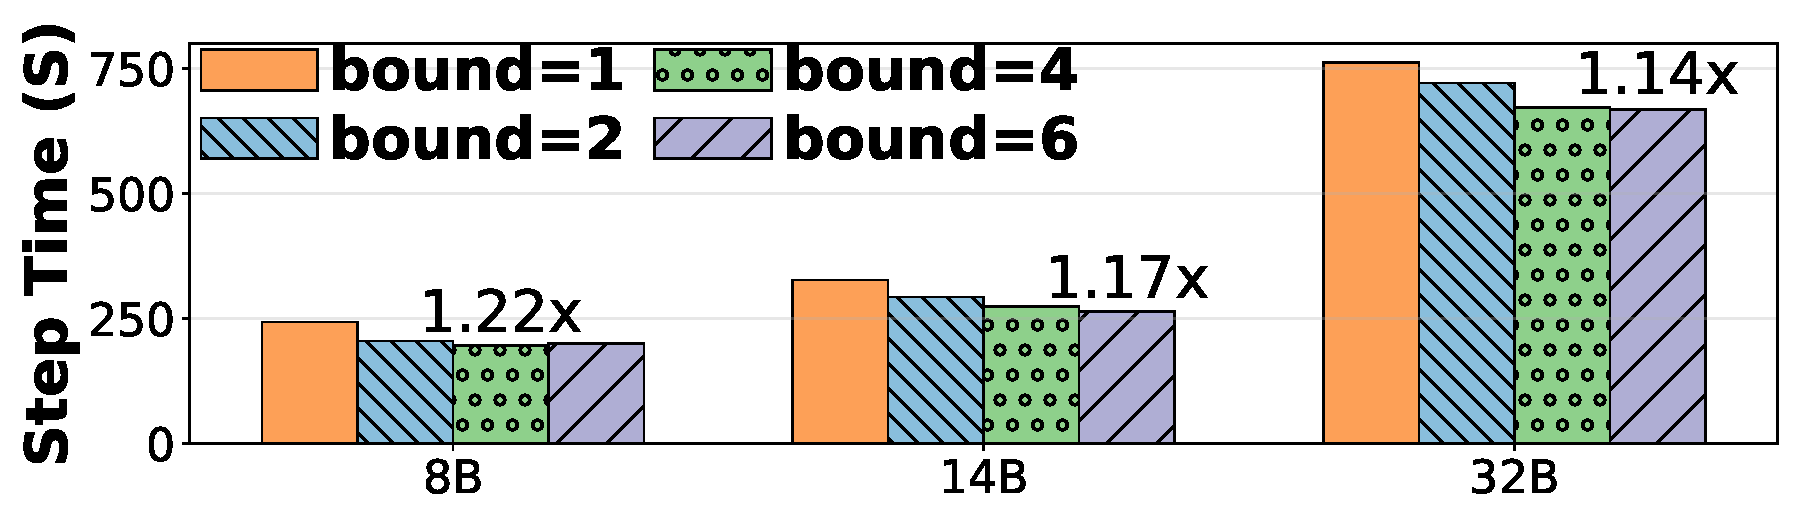
\includegraphics[width=0.9\linewidth]{figs/async_train/async_ratio.pdf}
    \vspace{-5pt}
    \caption{\textbf{[Principle 2]}: The average step time comparison of different asynchronous bounds across LLMs.}
    \label{fig:async-ratio}
\end{figure}


\subsection{Analysis of Trajectory-level Asynchrony}
\label{subsec:eval-async}
\noindent\textbf{Asynchronous Environment Interaction.} Trajectory-level environment management enables asynchronous environment interaction. We run Qwen3-8B/32K and inject additional environment latency sampled from gaussian distributions with mean \(\mu = 10\) and standard deviation \(\sigma\) ranging from 1 to 10 at each turn. We compare trajectory-level and batch-level interaction in \autoref{subfig:async_env_batch}, reporting the average step time over ten iterations. As the latency variance increases, the performance gains of trajectory-level over batch-level interaction grows from \(1.23\times\) to \(2.27\times\), proving asynchronous environment interaction sustains high throughput.

\noindent\textbf{Redundant Environment Rollouts.} GRPO exposes two key configuration parameters: the number of environment groups and the group size. By launching additional environments, redundant rollouts can tolerate environment failures and accelerate training. We run Qwen3-8B/32K on 32 H800 GPUs and vary both the number of environment groups and the group size on the \texttt{GEM-math} agentic task, reporting rollout speedup ratios in \autoref{subfig:env-red-rollout}. The maximum speedup reaches \(1.62\times\), and increasing either parameter yields positive speedup.

\noindent\textbf{Impact of Asynchrony Bound.}
We vary the asynchronous bound from 1 to 6 and report the average step time across LLMs in \autoref{fig:async-ratio}. Increasing the bound typically reduces the probability of aborting completed trajectories due to staleness, which in turn lowers the step time in most cases. However, we observe that efficiency plateaus within certain ranges. The optimal bound differs across LLMs and yields at most a 1.22\(\times\) step time reduction compared with a bound of 1. Considering overall training performance, these throughput gains do not necessarily translate into better time-to-score. In practice, setting the bound to one delivers satisfactory performance.

\begin{figure}[tb]
    \centering
    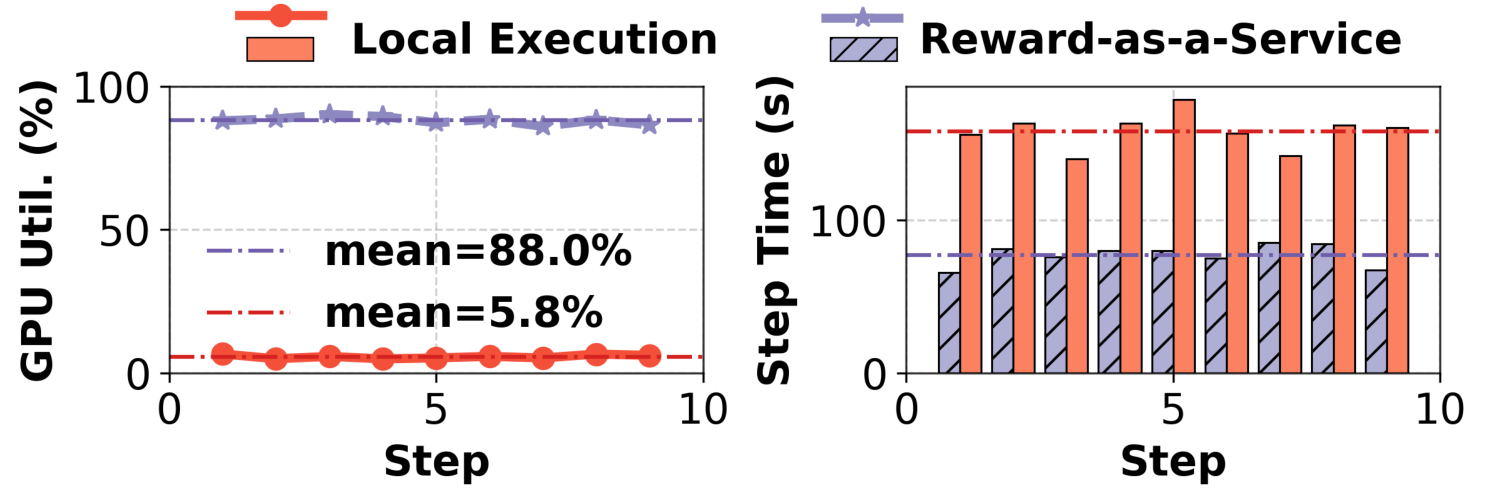
\includegraphics[width=\linewidth]{figs/reward/7B_experiments_comparison.pdf}
    \vspace{-15pt}
    \caption{\textbf{[Principle 3]}: Comparison between dedicating local GPUs and using Reward-as-a-Service.}
    \label{fig:reward_comparison_exp}
    % \vspace{-5mm}
\end{figure}

\begin{figure*}[tb]
    \centering
    \begin{subfigure}[b]{0.33\linewidth}
        \centering
        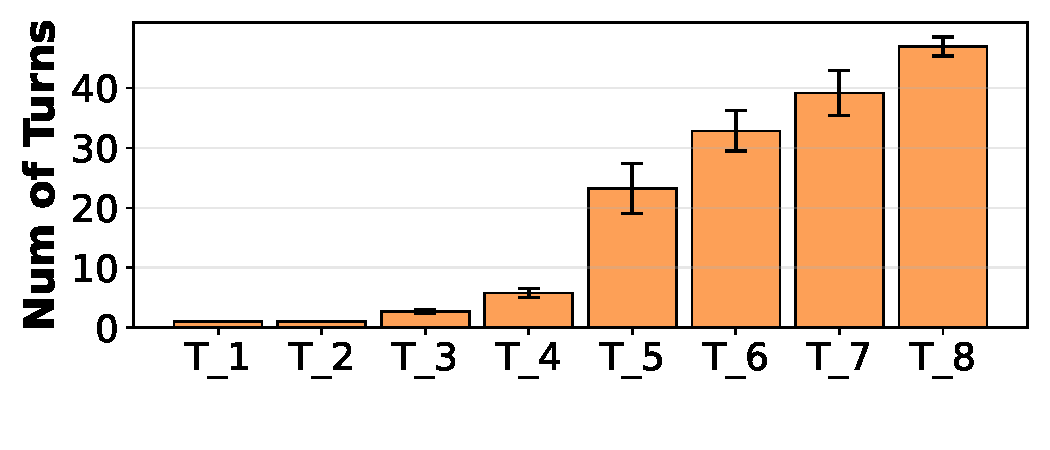
\includegraphics[width=\linewidth]{figs/trace/action.pdf}
        \caption{Average Number of Turns per Task.}
        \label{fig:action}
    \end{subfigure}
    % \hfill
    \begin{subfigure}[b]{0.33\linewidth}
        \centering
        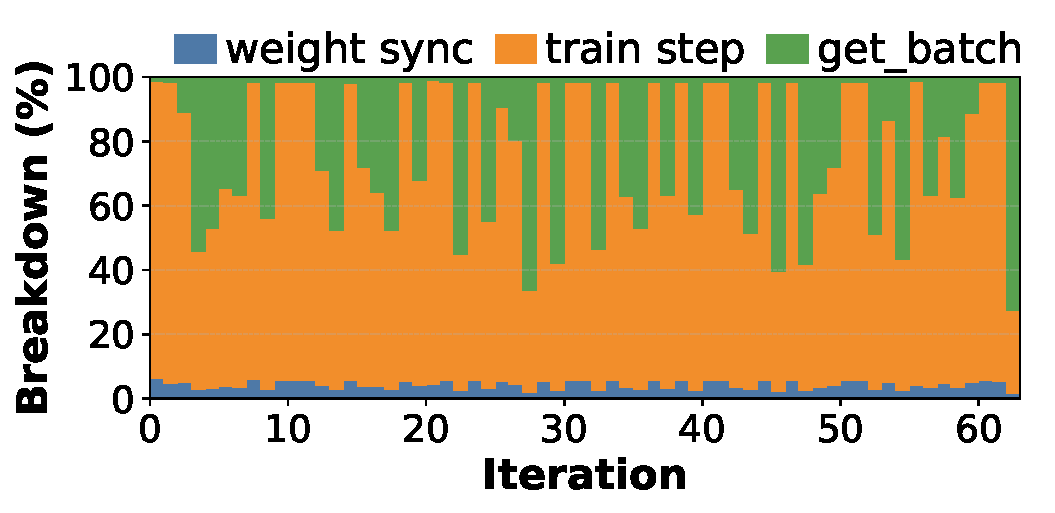
\includegraphics[width=\linewidth]{figs/trace/trace_dist.pdf}
        \caption{Step Time Distribution.}
        \label{fig:trace_dist}
    \end{subfigure}
    \begin{subfigure}[b]{0.33\linewidth}
        \centering
        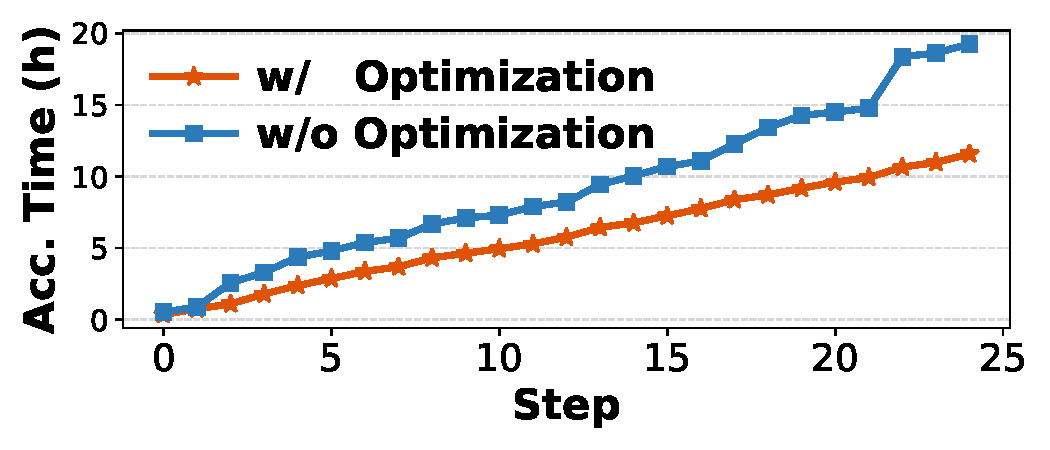
\includegraphics[width=\linewidth]{figs/trace/total_iter_time.pdf}
        \caption{Accumulated Step Time.}
        \label{fig:opt_step_time}
    \end{subfigure}
    \caption{Production-Grade Agentic RL Workload Characterization.}
    \vspace{-10pt}
    \label{fig:workload_overview}
\end{figure*}

\subsection{Benefits of Serverless Reward Worker}
\label{subsec:eval-reward-worker}
We evaluate \textit{Reward-as-a-Service} by comparing it with a dedicated local GPU setup. We run three concurrent agentic RL jobs on mathematical tasks with Qwen3-8B/16K as the agent and Qwen2.5-7B as the reward LLM on a 16-GPU cluster, using eight GPUs for training. In the local setup, four GPUs are reserved for the reward LLM. \autoref{fig:reward_comparison_exp} shows GPU utilization and rollout time per step for a batch size of 84, where rollout time includes asynchronous reward computation. The serverless platform is shared by three jobs and perform autoscaling, increasing average GPU utilization from 6\% to 88\%. Without the hot-standby GPUs for reward computation, more GPUs can be utilized for rollouts. Thus, the average rollout time reduces from 158 seconds to 77 seconds, demonstrating the benefits of statefulness-aware computation.
